\documentclass[11pt]{article}
\usepackage{fullpage}
\usepackage[margin=1.0in]{geometry}                % See geometry.pdf to learn the layout options. There are lots.
\geometry{letterpaper}                   % ... or a4paper or a5paper or ... 
%\geometry{landscape}                % Activate for for rotated page geometry
%\usepackage[parfill]{parskip}    % Activate to begin paragraphs with an empty line rather than an indent
\usepackage{graphicx}
\usepackage{amssymb}
\usepackage{amsmath}
\usepackage{algorithmic}
\usepackage{epstopdf}
\DeclareGraphicsRule{.tif}{png}{.png}{`convert #1 `dirname #1`/`basename #1 .tif`.png}
\usepackage{tikz}
\usetikzlibrary{positioning}
\newcommand{\LD}{\langle}
\newcommand{\RD}{\rangle}



\title{}
\author{}
\date{}                                           % Activate to display a given date or no date

\begin{document}

\maketitle
%\section{}
%\subsection{}

\section{Sort using heaps}
\begin{itemize}
\item{
Give an $O(n\,log\,k)$ algorithm to merge k sorted lists with n total elements into one sorted list.
\\
\\
Let ${l_1, l_2, \dots,l_k}$ be the set of sorted lists. Refer to the elements of a given list $l_i$ using array notation, so for example ${l_i}[0]$ is the first element of $l_i$.
\\
\begin{algorithmic}
  \STATE Create empty min-heap, $H$
  \FOR{$1$ to $k$}
  \STATE Make a key-value pair , $v = ({l_i}[0], l_i)$
  \STATE Insert($H$,$v$)
  \ENDFOR
  \STATE Create empty sorted list, $S$.
  \WHILE{$H$ is not empty}
    \STATE Let $x$ = pop(the list at ($H,root$)) \COMMENT{Pop off the list's first item, not the list itself}
    \STATE inject($S$, $x$)
    \IF{size(the list at ($H,root$)) = 0}
      \STATE Extract-Min($H, root$) \COMMENT{Simply discard empty list}
    \ELSE
      \STATE Update the key at ($H,root$) to be head(the list at ($H,root$))
      \STATE Min-Heapify($H,root$)
    \ENDIF
  \ENDWHILE
\end{algorithmic}

The keys in the heap are always the smallest values currently in each $l_i$ since each list is sorted. Because $H$ is a min-heap, the key at the root is the smallest value over all lists in the heap. All smaller values have already been removed and appended to $S$.
\\
\\
The initial for loop is $O(k\,log\,k)$ because $k$ lists are inserted into the heap. The while loop executes $n$ times, appending the next smallest item to $S$ on each iteration. Each iteration calls either Extract-Min or Min-Heapify, which take $O(log\,k)$ time. Thus the while loop is $O(n\,log\,k)$.
}

\newpage

\item{
Give an $O(n\,log\,k)$ algorithm to for sorting a list of $n$ numbers that is $k$-close to sorted.
\\
\\
In this discussion I will use the following terminology: For a given item that belongs at index $i$ of the list, the item is ``to the left'' of its proper index $i$ if it is currently at index $j < i$, and the item is ``to the right'' of $i$ if it is currently at index $j > i$. In other words I imagine the list in the standard way, with its positions ${1,2,\dots,n}$ in ascending order from left to right. \\
Also note that I will index the list from $1,\dots, n$ instead of from $0\dots n-1$.
\\
\\
Let $S$ be a list that is $k$-close to sorted, and let $s_1,s_2,\dots, s_n$ be the items that belong at positions $1,\dots, n$ respectively. \\
By definition, for a given index $i$ of the list, the item $s_i$ that belongs at position $i$ cannot be further than $k-1$ positions to the right of $i$. Specifically, consider the item that belongs at position 1, $s_1$.  There are no positions to the left of 1, so $s_1$ must be at one of the positions between 1 and $k$.
\\
\\
Furthermore, suppose there is an index $j$ such that all items to the left of $j$ are 1-close to sorted - they are in their proper positions - and all items from $j,\dots,n$ are $k$-close to sorted. Then $s_j$ must be at one of the positions from $j,\dots,(j+k-1)$. In this scenario $s_j$ cannot be at one of the positions from $(j-k+1)\dots, (j-1)$, even though that would meet the definition of $k$-close to sorted, because if it were then there would be some other item in that range that was not 1-close to sorted.
\\
\\
I will rely on these facts in the algorithm below: 
\\
\begin{algorithmic}
\STATE Add $k$ extra empty spaces onto the tail end of the list $S$ \COMMENT{now it has indices $1,\dots,(n+k)$}
\STATE Build a min-heap $H$ with the sublist of $S$ at indices $1,\dots,k$
\FOR{$i={(k+1)}$ \TO $n$}
	\STATE Swap the item at position 1, the root of $H$, with the item at position $i$
	\STATE Min-Heapify($H,root$)
\ENDFOR
\STATE Return pointer to index $k+1$ of $S$ \COMMENT{starting index of the fully sorted list}
\end{algorithmic}

Since the smallest item in $S$, $s_1$, starts out somewhere from $1,\dots,k$, it follows that after initially building the min-heap on indices $1,\dots,k$, $s_1$ is at the root of $H$ (at position 1). \\
Then the for loop begins. The list currently has the scenario described above with $j=2$, where items to the left of 2 are fully sorted, and the items starting at position 2 and to the right are $k$-close to sorted. This means that $s_2$ must be in one of the positions from $2,\dots,(k+1)$. \\
The swap puts $s_1$ into its final position, $k+1$, and the item that was at $k+1$ to the root of $H$. To maintain the heap ordering the algorithm calls Min-Heapify($H,root$). Now the item at the root of $H$ is $s_2$. \\
The next iteration of the for loop starts and moves $s_2$ into its final position, $k+2$. After $n$ iterations the list is fully sorted and ranges from $(k+1),\dots,(n+k)$.

This method requires $O(k)$ additional space for the extra spaces at the end of the list. \\
Building the heap out of indices $1,\dots,k$ requires $O(k\,log\,k)$ (loose) or $O(k)$ (tight) time. Then the for loop executes $n-k = O(n)$ times and does $O(log\,k)$ work each time when it calls Min-Heapify. Thus it is $O(n\,log\,k)$.


}

\end{itemize}

\section{Longest path in a DAG}

The algorithm should start by performing topological sort on the DAG. The longest path will start at a source and end at a sink, except for the cases when all edges emanating from the source(s) are negative and when all edges entering the sink(s) are negative. Even in those cases it still works to examine the edges in topological order because the longest path still has the form $v_1,\dots,v_k$ where the $v_i$s occur in topological order. (This is true even if the longest path is 0, for just a single node.)
\\
\\
After initializing the distance of each vertex to 0, the algorithm next goes through the vertices in topological order and checks each edge $(v,w)$ emanating from the current vertex $v$. If the path through $v$ to a given $w$ is longer than the longest known path to $w$ then it updates the distance to $w$ with this larger value, and updates $w$'s ``prev'' pointer to $v$. \\
\\
Two observations: First, because all distances are initialized to 0, negative paths to $w$ will never overwrite the currently longest known path to it. Second, because the vertices are examined in topological order, all edges into a given vertex $w$ have been checked before calculating the distances of vertices reachable \emph{from} $w$. Therefore since we know the longest path \emph{to} $w$, distances to vertices $x$ reachable through edges $(w,x)$ are also maximized. \\
\\
Here is pseudocode:
\begin{algorithmic}
\STATE order[]
\STATE Perform topological sort on G using DFS
\STATE Populate order[] with $v \in V$ in topological order (decreasing postorder number)
\STATE dist[]
\STATE prev[]
\STATE longest\_path := 0
\STATE longest\_path\_end := order[0]
\FORALL{$v \in V$}
	\STATE dist[$v$] := 0
\ENDFOR
\FOR{$v$ in order[]}
	\FORALL{$(v,w)$}
		\IF{dist[$w$] $<$ dist[$v$] + length$(v,w)$}
			\STATE prev[$w$] := v		
			\STATE dist[$w$] := dist[$v$] + length$(v,w)$
			\IF{dist[$w$] $> longest\_path$}
				\STATE $longest\_path$ := dist[$w$]
				\STATE $longest\_path\_end$ := $w$
			\ENDIF
		\ENDIF
	\ENDFOR
\ENDFOR
\STATE Find the longest path by starting with $longest\_path\_end$ and tracing back through prev[] 
\end{algorithmic}

\flushleft{DFS takes time $O(|V| + |E|)$.} The second part of the algorithm is also $O(|V| + |E|)$ because it runs over all vertices and edges doing constant work. The final extraction of the longest path is $O(|V|)$, so the algorithm as a whole is $O(|V| + |E|)$.

\section{Short Answer}
\begin{itemize}
\item{
Consider a depth first search on the graph below starting at vertex A. \\
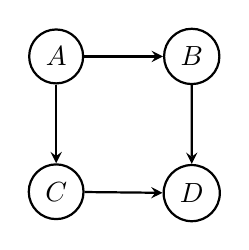
\begin{tikzpicture}[xscale=6, yscale=8,>=stealth]
\tikzstyle{v}=[circle, minimum size=1mm,draw,thick]
\node[v] (a) {$A$} [label=left:$ 1\ 8 $];
\node[v] (b) [right=of a] {$B$};
\node[v] (c) [below=of a] {$C$};
\node[v] (d) [below=of b] {$D$};
\draw[thick,->]
(a) to node {} (c);
\draw[thick,->]
(a) to node {} (b);
\draw[thick,->]
(b) to node {} (d);
\draw[thick,->]
(c) to node {} (d);
\end{tikzpicture}

The DFS would assign the following [preorder, postorder] pairs: \\
A: [1,8] \\
B: [2,5] \\
C: [6,7] \\
D: [3,4] \\
Arranging these in order by decreasing postorder number, A, C, B, D, yields a valid topological ordering. Ordering them by preorder number, A, B, D, C, does not. The problem is that there are disjoint pre and postorder intervals ([3,4] and [6,7]).
}

\item{
The running time of DFS using an adjacency matrix representation is $O(n^2)$ where $n$ is the number of vertices in the graph. One call of search($v$) is $O(n)$ because it must check for edges in all $n$ columns of $v$'s row in the matrix. The DFS procedure calls search $n$ times, so overall it is $O(n^2)$.
}

\end{itemize}

\section{Buffy's Patrol}

\par{Imagine Sunnydale as a graph where edges are streets and vertices are intersections. Assume that it is possible to patrol both sides of every street. That is, the city is an undirected graph or a directed graph where every edge $(u,v)$ has a corresponding edge $(v,u)$. In addition to true intersections, consider dead ends to be vertices, and treat any point where a street leaves Sunnydale as a vertex. Finally assume that the city-graph is connected. Starting at any intersection there is some path to every other intersection.}

\par{Buffy can use a modified version of DFS to patrol each street once on each side. Basically the algorithm is "walk out as far as you can, then come back on the other side." To make it more precise I introduce a new operation on edges, traverse$(u,v)$, which simply means walk from $u$ to $v$. Similarly traverse($v$,$u$) means walk (back) to $u$. }
\\ Here is an edited search($v$):
\begin{algorithmic}
\STATE explored($v$) := 1
\FOR{$(v,w) \in E$}
\IF{explored($w$) = 0}
\STATE traverse($v,w$)
\STATE prev[$w$] := $v$
\STATE search($w$)
\ELSIF{traversed[($v,w$)] = 0} 
\STATE traverse($v,w$)
\STATE traverse($w,v$)
\ENDIF
\ENDFOR
\end{algorithmic}

\par{The search procedure updates two new lists, prev and traversed. prev holds a pointer for each vertex $v$ to the vertex $u$ to which Buffy should walk on her way \emph{back}. traversed holds a flag for each edge indicating whether Buffy has already walked it or not. Notice that order matters, Buffy may have traversed $(u,v)$ but not $(v,u)$. The explored list is the same as in the class version of search($v$), a list of flags for each vertex.}
\par{Using this procedure, Buffy will walk out along one side of every street. Any time she sees an finds a street that leads to an intersection she has already visited, she just walks down that street to the intersection and comes back. Thus the ``going out'' portion is covered with the class DFS procedure and this modified search procedure. To finish the patrol, any time there are no unexplored vertices nor untraversed edges from her current vertex $w$ Buffy should return to prev[$w$], i.e. traverse($w$,prev[$w$]), walking along the other side of the street.}

\section{Djikstra's algorithm for non-negative integer edge costs}
Give an algorithm that finds shortest paths in $O(|E| + |V|m)$ where $m$ is the largest edge cost.
I don't have a full solution to this problem, but here are some ideas: \\
Dijkstra's algorithm is $O(|E| * Insert + |V| * Delete-Min)$. Therefore an algorithm with an Insert that runs in $O(1)$ time and a Delete-Min that runs in $O(m)$ time solves the problem.
\\
\par{That points to a data structure that uses a list, because inserting into a linked list is $O(1)$. Data structures that are sorted or partially ordered cannot insert in $O(1)$ time.} \\
\par{Also, it is possible to find the minimum of $m$ elements in $m$ steps, so this data structure should make it possible to only look at $m$ elements during each Delete-Min operation.}
\par{Therefore, assuming $m$ is known ahead of time, a possible data structure is an array of size $m +1$, with indices ${0,\dots,m}$, where each element of the array is a pointer to a list of vertices. Suppose whenever the algorithm finds an edge $(v,w)$ with cost $c\ (0 \le c \le m)$, $w$ is inserted onto the list pointed to by index $c$ of the array. That is, every vertex is put into one of $m+1$ buckets.}
\par{If we could be certain that each vertex in a given bucket is interchangeable with the other vertices in that bucket, then Delete-Min could operate by checking the distance to the first item in each of the $m+1$ lists, keeping a running pointer to the element with the minimum distance. Then it could delete that list element in $O(1)$ time, so Delete-Min would be $O(m)$. Since Delete-Min would have to be run $|V|$ times to delete every vertex, over the course of the algorithm it would be $O(|V|m)$.}

\newpage
\section{Shortest Path Verification}
\par{Suppose that you are given a directed graph G = (V,E) along with weights on the edges (you can assume that they are all positive). You are also given a vertex s and a tree T connecting the graph G that is claimed to be the tree of shortest paths from s that you would get using Dijkstra's algorithm. Can you check that T is correct in linear time?}
\par{Yes, the algorithm below is $O(|E| + |V| + |T|)$. First it gathers up the shortest distances to each vertex supplied by the tree T, which takes time $O(T)$. Then for every vertex $v$ it checks if there is an edge $(v,w)$ that implies a shorter path to $w$ than what T offers. This part has a bound of $O(|V| + |E|)$. If any shorter path is found it returns false (the given tree in not the set of shortest paths). Otherwise it returns true.}
\begin{algorithmic}
\STATE create dist[]
\STATE dist[s] := 0
\STATE create queue q
\STATE inject(q,s)
\WHILE{size(q) $>$ 0}
\STATE v := eject(q)
\FORALL{(v,w) $\in$ T}
\STATE dist[w] := dist[v] + length(v,w)
\STATE inject(q,w)
\ENDFOR
\ENDWHILE
\FORALL{v $\in$ V}
\FORALL{(v,w) $\in$ E}
\IF{dist[v] + length(v,w) $<$ dist[w]}
\STATE return false \COMMENT{found a shorter path}
\ENDIF
\ENDFOR
\ENDFOR
\STATE return true
\end{algorithmic}
\newpage
\section{Risk Free Currency Exchange}
Model the problem with a directed graph: Treat each currency $c_{i}$ as a vertex. There is a directed edge $(c_{i},c_{j})$ between every currency that has edge cost $r_{i,j}$. So if you start with one unit of $c_{i}$ and travel the edge to $c_{j}$, you obtain $r_{i,j}$ units of $c_{j}$. Traveling down another edge $(c_{j},c_{k})$ that has weight $r_{j,k}$ results in $r_{i,j} * r_{j,k}$ units of $c_{k}$. \\
The task is then to find a cycle $c_{i},c_{j},\dots,c_{i}$ whose product $r_{i,j} * r_{j,k} * \cdots * r_{l,i} > 1$. Or for the purposes of this problem simply to detect whether such a cycle exists. The algorithm below uses a modified search procedure that passes through a running product value. The product gets updated on each recursive call. At any point when a cycle is found (i.e. when a back edge is found), it checks if the product is $>$ 1 when following the back edge, and if so returns true. \\
This algorithm has the same running time as DFS, $O(|E| + |V|)$, because it only adds constant work to each call of search($v$). \\
\begin{algorithmic}
\STATE Procedure search($v$, product)
\STATE explored($v$) := 1
\IF{explored($w$) = 0}
\STATE product := product $*\ r_{v,w}$
\STATE search($w$,product)
\ELSE
\IF{product * $r_{v,w} > 1$}
\STATE return true \COMMENT{Back edge found and it yields product $>$ 1}
\ENDIF
\ENDIF
\STATE End search
\end{algorithmic}
Then search is used in DFS just as in the class version except for passing product. This DFS also initializes product to 1 after each restart: \\
\begin{algorithmic}
\STATE Procedure DFS $(G(V,E))$
\FORALL{$v \in V$}
\STATE explored($v$) := 0
\ENDFOR
\FORALL{$v \in V$}
\IF{if explored($v$) = 0}
\STATE product := 1
\STATE search($v$, product)
\ENDIF
\ENDFOR
\STATE End DFS
\end{algorithmic}
\end{document}  
